\documentclass[a4paper,14pt]{extreport}
\usepackage[utf8]{inputenc}
\usepackage[english,russian]{babel}
\linespread{1.3}
\usepackage[left=3cm, right=1.5cm, top=2cm, bottom=2cm, bindingoffset=0cm]{geometry}
\usepackage{indentfirst}
\usepackage{amsmath,amssymb,amscd,amsfonts,amsthm}
\usepackage{graphicx}
\usepackage[hidelinks]{hyperref}
\usepackage{titlesec}
\usepackage{listings}
\usepackage{tikz}
\usepackage{pgfplots}
\usepackage{ccaption}
\usepackage{floatrow}
\usepackage{listings}
\usepackage{xcolor}
\titleformat{\chapter}[display]{\filcenter}{\large\MakeUppercase{\chaptertitlename} \thechapter}{8pt}{\large\bfseries}{}
\titleformat{\section}{\large\bfseries}{\thesection.}{1em}{}
\titleformat{\subsection}{\normalsize\bfseries}{\thesubsection.}{1em}{}
\titlespacing*{\chapter}{0pt}{-30pt}{18pt}
\titlespacing*{\section}{\parindent}{18pt}{18pt}
\titlespacing*{\subsection}{\parindent}{18pt}{18pt}
\newtheorem{theorem}{\hspace{\parindent}Теорема}[chapter]
\newtheorem{lemma}{\hspace{\parindent}Лемма}[chapter]
\newtheorem{statement}{\hspace{\parindent}Утверждение}[chapter]
\theoremstyle{definition}
\newtheorem{definition}{\hspace{\parindent}Определение}[chapter]
\newtheorem{example}{\hspace{\parindent}Пример}[chapter]
\newtheorem{algorithm}{\hspace{\parindent}Алгоритм}[chapter]
\newtheorem{remark}{\hspace{\parindent}Замечание}[chapter]
\renewcommand{\large}{\fontsize{17}{20pt}\selectfont}
\renewcommand{\Large}{\fontsize{20}{25pt}\selectfont}
\lstdefinestyle{sharpc}{language=[Sharp]C,  rulecolor=\color{black}}

\pgfplotsset{test1/.style = {red}}
\pgfplotsset{test2/.style = {blue}}
\pgfplotsset{test3/.style = {green}}
\pgfplotsset{test4/.style = {black}}
\lstset{keepspaces = true}

\makeatletter
\renewcommand{\@biblabel}[1]{#1.}
\makeatother


\begin{document}
\begin{titlepage}
\thispagestyle{empty}
\begin{center}

МИНИСТЕРСТВО ОБРАЗОВАНИЯ И НАУКИ РФ

БУРЯТСКИЙ ГОСУДАРСТВЕННЫЙ УНИВЕРСИТЕТ

Институт математики и информатики

Кафедра прикладной математики
\end{center}

\vspace{2 cm}
\begin{center}
Курсовая работа
\end{center}
\begin{center}
\Large Моделирование деревьев \linebreak в СУБД MySQL
\end{center}
\vspace{3em}
\begin{table}[h!]
\begin{tabular}{p{0.45\linewidth}l}
\hfill Выполнил: & студент 4 курса группы 05230\\
                        & Саяпин Никита Александрович \\
\hfill Научный руководитель: & ст.преп. кафедры ПМ, к.ф-м.н \\
                        & Трунин Дмитрий Олегович \\
\hfill Научный консультант: & ст.преп. кафедры ИТ \\
                        & Хабитуев Баир Викторович \\
\end{tabular}
\end{table}
\vspace{\fill}
\begin{center} Улан-Удэ \\ 2016
\end{center}
\end{titlepage}
\setcounter{page}{2}
\tableofcontents{}
\chapter*{ВВЕДЕНИЕ}
\addcontentsline{toc}{chapter}{Введение}
Дерево - это структура данных, которая представляет собой древовидную структуру в виде набора связанных узлов, и являющаяся связным графом, не содержащим в себе циклов\cite{Kormen}.

Данная структура благодаря своей простоте и удобству получила широкое применение в практических целях. В настоящее время многие информационные системы применяют в работе деревья. Они предназначены для хранения информации о списках друзей, комментариев к какой-либо новостной статье, для реализации списка участников бонусных программ и других задач. Однако при создании структур данного класса программисты чаще всего сталкиваются с проблемой быстродействия кода. Не секрет, что при достаточно большом объеме данных многие базы данных, хранящие в себе деревья, начинают проявлять сбой в работе. Поэтому основной задачей разработчиков является разработка таких программных систем для работы с данными, которые позволяют выполнить операции для работы с деревьями за как можно меньшее время.

Целью работы является реализация системы для генерации структур типа «Деревья» на языке программирования PHP\cite{PHP,Zandstra} с использованием системы управления базами данных MariaDB, которая является свободно распространяемой версией широко применяемой на практике системы управления базами данных MySQL\cite{MySQL,Schwartz}.

В рамках курсовой работы были поставлены следующие задачи:
\begin{enumerate}
\item Изучение и рассмотрение основных структур хранения деревьев в базах данных.
\item Программная реализация основных операций для работы с данными, хранящимися в различных типах дереьев.
\item Реализация и тестирование программного кода.
\end{enumerate}

Курсовая работа состоит из введения, трех глав, заключения, списка литературы и
приложения.

\chapter{Основные структуры хранения деревьев в базе данных}
\section{Введение в хранение простых деревьев}
Рассмотрим задачу хранения данных в дереве на конкретном примере.

Допустим, что мы разрабатываем некоторую систему хранения комментариев, в которой каждый пользователь может оставлять комментарии или отвечать на уже написанный комментарий. Перед нами стоит задача отслеживания цепочки ответов пользователей в данной системе, в котором каждый комментарий в зависимости от ситуации может ссылаться на один из комментариев или быть независмым от других комменатриев. Для хранения комменатриев мы используем базы данных, а для реализации связей применяются структуры деревьев. Однако тут же возникает следующий вопрос: каким образом можно хранить связи между элементами в базе данных?

Существуют четыре основные структуры хранения деревьев в базах данных\cite{Karwin}:
\begin{enumerate}
\item Список смежности(Adjacency List), хранящий информацию об узле и его родителе;
\item Перечисление путей(Materialized Path), который в каждом узле содержит информацию о пути от вершины дерева к данному узлу;
\item Вложенные множества(Nested Sets), структура, каждый элемент которой имеет два номера, которые идентифицируют ее как узел дерева, а также уровень вложенности соответствующего узла;
\item Таблица замыканий(Closure Table), структура, которая реализуется с помощью двух таблиц в базе данных, и содержит в каждом узле информацию не только о родителях данного узла и уровне вложенности, но и информацию о все родительской ветке для данного узла.
\end{enumerate}
В рамках курсовой работы были реализованы все четыре основных метода реализации дереьев в среде MySQL/MariaDB. Помимо этого, описаны преимущества и недостатки каждой из структур.
\section{Информация об основных структурах реализации деревьев}
В данной подглаве мы рассмотрим основные структуры хранения деревьев в базах данных, а также рассмотрим проектирование таблиц базы данных для СУБД MySQL.

В таблицах СУБД MySQL приняты соответствующие обозначения полей:

\subsection{Список смежности}
Эта структура содержит в себе представление о коллекции списков вершин, иначе говоря, каждой вершине дерева соответствует список, состоящий из узлов, которые связаны с данным\cite{Groshev}.  Для того, чтобы реализовать ее, нам достаточно знать лишь информацию о том, к какому узлу ссылается текущий узел, или другими словами, связь между узлом и его родителем.

Соответственно, для практической реализации данной структуры нам достаточно занести в соответствующую таблицу базы данных два поля: идентификатор узла дерева и идентификатор его родителя\cite{Ermakov}.

Метод является одним из наболее простых для реализации деревьев. На практике он применяется во многих задачах, в частности, для хранения списка непосредственного списка друзей, списка комментариев и многих других задач, которые применяют для реализации древовидные структуры.
\begin{figure}[h!]
\begin{center}
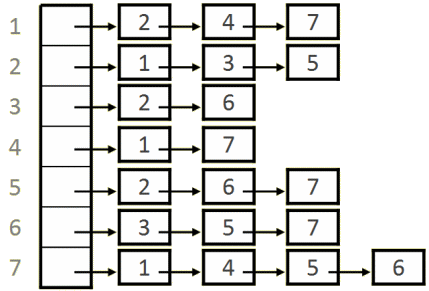
\includegraphics[width=8cm]{11.png}
\caption{Примерный графический вид структуры "Список смежности" в таблице СУБД MySQL}
\label{fig:3}
\end{center}
\end{figure}
Для удобства работы с методом доработаем таблицу, добавив в него два соответствующих поля: поле для хранения имени пользователя, а также поле статуса пользователя, которое показывает, заблокирован ли пользователь в системе или нет. Данное решение более предпочтительно, чем удаление пользователя из дерева, так как позволяет в кратчайшие сроки при возможности восстановить его. В таблице 1.1 показана изображена структура таблицы базы данных, реализующая данную структуру.

\begin{table}[H]
\ttabbox{\caption{Структура таблицы базы данных, реализующей структуру 'Список смежности'}
\label{tab:1}}{
\begin{tabular}{ | c     | c     | c    | }
\hline
Атрибут & Тип & Описание\\ \hline
   user\_id     &   int(11)   &  Идентификатор узла в структуре решения      \\ \hline
   parent\_id     &    int(11)    & Идентификатор родительского узла     \\ \hline
   user\_name    &    varchar(255)    & Имя узла       \\ \hline
   user\_status     &    char(1)    &  Статус(свойство) узла     \\ \hline

\end{tabular}}
\end{table}
\subsection{Перечисление путей}
Данный метод экономно решает задачу извлечения предков заданного узла в дереве. Он хранит в себе поле, которое в каждом узле содержит путь, который начинается с родительского узла, не имеющего предков, и заканчивается в данном узле. Между ними находятся узлы, которые соединяют родительский узел с текущим.
Данный метод удобен для организации иерархических структур, с его помощью можно легко вывести все комментарии к записи или каталог всех товаров, которые продаются на предприятии.
\begin{figure}[h!]
\begin{center}
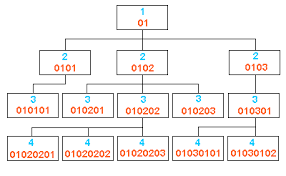
\includegraphics[width=8cm]{12.png}
\caption{Примерный графический вид структуры "Список смежности" в таблице СУБД MySQL}
\label{fig:3}
\end{center}
\end{figure}
Реализация алгоритма перечисления путей аналогична алгоритму списка смежности, только вместо поля хранения информации о родителе узла мы добавляем поле, в котором содержится путь для данного узла.

\begin{table}[H]
\ttabbox{\caption{Вид метода хранения деревьев 'Перечисление путей' в таблице СУБД MySQL}
\label{tab:1}}{
\begin{tabular}{ | c     | c     | c    | }
\hline
Атрибут & Тип & Описание\\ \hline
   user\_id     &   int(11)   &  Идентификатор узла в структуре решения      \\ \hline
   user\_name    &    varchar(255)    & Имя узла       \\ \hline
   user\_path    &    varchar(255)    & Путь к узлу, начиная с корня дерева     \\ \hline
   user\_status     &    char(1)    &  Статус(свойство) узла     \\ \hline

\end{tabular}}
\end{table}
В процессе работы с данной структуры можно столкнуться с некорректной сортировкой путей. Дело в том, что поле, которое хранит путь в таблице базы данных, является строковым. Поэтому оно сортирует поле в алфавитном порядке, а не в числовом. Так например, при сортировке данных по пути после узла с полем '/1' может стоять узел, содержащий в себе путь '/1/10', а не '/1/2'. Для того, чтобы избежать подобной проблемы, применяются различные доработки базы данных. Одним из наиболее простых способов решения является добавление параметра UNSIGNED ZEROFILL  для идентификатора данного узла. Данный параметр автоматически дополняет нулями данный идентификатор до того количества символов, которым ограничено данное поле в таблице. Тогда путь будет содержать информацию о связях узлов с учетом данного параметра. Недостатком данной доработки являются ограничения на длину идентификатора пользователя и пути, которые не позволяют вставлять узлы ниже определенного уровня, а также узлы, номер которых содержит в себе цифр больше, чем может вместить в себя идентификатор.

\subsection{Вложенные множества}
Данное решение по хранению деревьев позволяет хранить информацию с каждым узлом, принадлежащим множеству его потомков, а не его непосредственным родителем. Данную информацю можно получить с помощью кодирования каждого узла с помощью двух номеров, левого и правого. Эти номера задаются следующим образом: левый номер меньше, а правый соответственно больше всех номеров дочерних объектов. Способом назначений левого и правого номера в этом методе состоит в выполнении прохода по всему дереву. Каждому узлу присваиваются значения левого номера с приращением при спуске по ветви дерева и значения правого номера при обратном подъеме по ветви\cite{Celco}.
\begin{figure}[h!]
\begin{center}
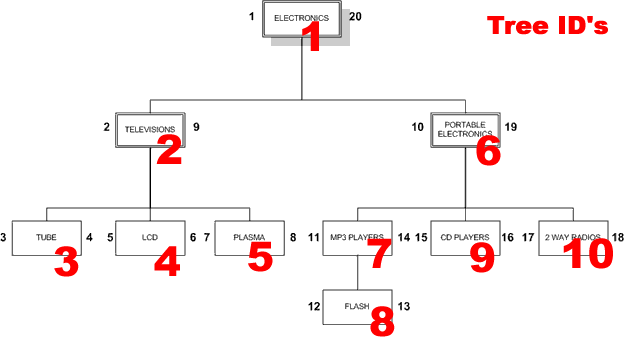
\includegraphics[width=8cm]{13.png}
\caption{Примерный графический вид структуры "Вложенные множества" в таблице СУБД MySQL}
\label{fig:3}
\end{center}
\end{figure}
При желании в таблицу можно также добавить и уровень вложенности текущего узла. Это поле показывает положение узла в текущей структуре дерева и определяется по минимальному количеству переходов от корня дерева до данного узла. Например, корневой узел '1' имеет уровень вложенности '1', а узел с идентификатором '3' , родителем которого является корневой узел '1' , имеет уровень вложенности "2".

Рисунок 1.3 показывает структуру данного решения в базе данных \\MySQL.
\begin{table}[H]
\ttabbox{\caption{Вид метода хранения деревьев 'Вложенные множества' в таблице СУБД MySQL}
\label{tab:1}}{
\begin{tabular}{ | c     | c     | c    | }
\hline
Атрибут & Тип & Описание\\ \hline
   user\_id     &   int(11)   &  Идентификатор узла в структуре решения      \\ \hline
   user\_name    &    varchar(255)    & Имя узла       \\ \hline
   left\_number   &    int(11)    & Левый номер узла     \\ \hline
   right\_number     &    int(11)    &  Правый номер узла     \\ \hline
   level    &    char(1)    &  Уровень вложенности узла     \\ \hline
   user\_status     &    char(1)    &  Статус(свойство) узла     \\ \hline

\end{tabular}}
\end{table}
\subsection{Таблица замыканий}
Этот метод является простым способом хранения иерархий в базе данных \cite{Tarasov}. В отличие от остальных методов, этот метод реализуется с помощью двух таблиц, а не одной. В первой таблице хранится информация об узлх дерева(в частности, там может зранится информация об имени и статусе узла). Во второй же таблице содержится вся информация о связях между элементами дерева, причем информация о связи между родителями и потомками заносится даже в том случае, если их разделяют несколько уровней, то есть таблица содержит информацию не только о непосредственном родителе данного узла, но и о предках данного родителя до корневого узла.

\begin{figure}[h!]
\begin{center}
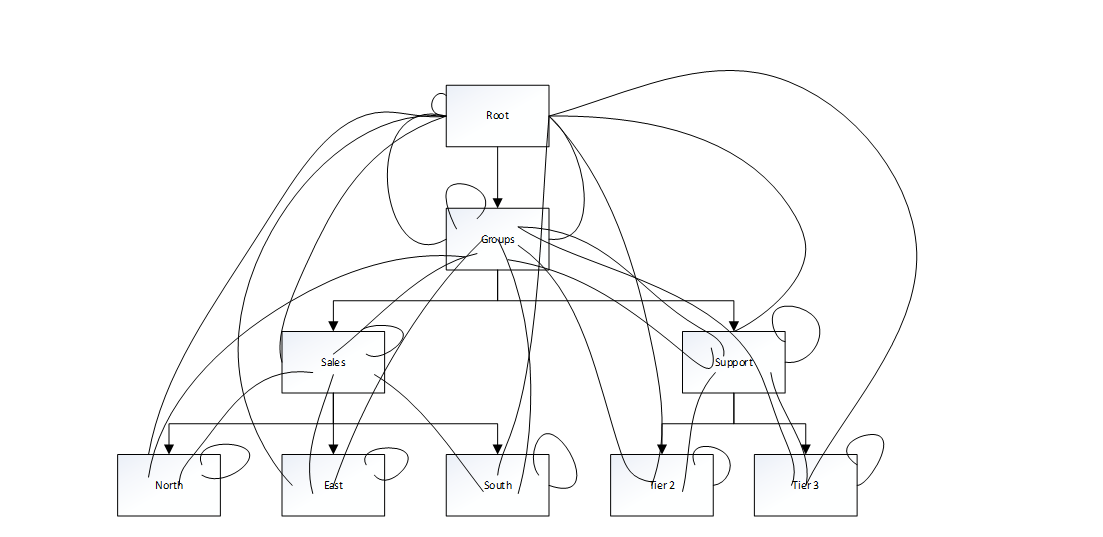
\includegraphics[width=12cm]{14.png}
\caption{Вид метода хранения деревьев "Таблица замыканий" в таблице СУБД MySQL}
\label{fig:3}
\end{center}
\end{figure}
 Помимо всего прочего, в таблице базы данных хранится ссылка на данный элемент, которая позволяет ссылаться на текущий узел. Так, например, нам нужно занести в базу данных информацию о связах узла 17, чьим предком является узел 10, который является ребенком узла 5, являющегося сыном коренного узла. Тогда в таблицу занесутся следующие записи(таблица 1.4):
\begin{table}[H]
\ttabbox{\caption{Вид вставляемых элементов в таблицу связей для метода 'Таблица замыканий'}
\label{tab:1}}{
\begin{tabular}{ | c     | c     | c    | }
\hline
user id & parent id & level \\ \hline
   17     &    1    &    4    \\ \hline
   17     &    5    &    3    \\ \hline
   17     &    10    &    2    \\ \hline
   17     &    17    &    1    \\ \hline
\end{tabular}}
\end{table}

В таблицах 1.5 и 1.6 изображено представление двух таблиц, реализующих данный метод хранения деревьев- таблицы, содержащей информацию об узлах дерева и таблицы,в которой лежит информация о связях между элементами соответственно.
\begin{table}[H]
\ttabbox{\caption{Таблица узлов метода хранения деревьев 'Таблица замыканий' в таблице СУБД MySQL}
\label{tab:1}}{
\begin{tabular}{ | c     | c     | c    | }
\hline
Атрибут & Тип & Описание\\ \hline
   user\_id     &   int(11)   &  Идентификатор узла в структуре решения      \\ \hline
   user\_name    &    varchar(255)    & Имя узла       \\ \hline
   user\_status     &    char(1)    &  Статус(свойство) узла     \\ \hline

\end{tabular}}
\end{table}
\begin{table}[H]
\ttabbox{\caption{Таблица связей метода хранения деревьев 'Таблица замыканий' в таблице СУБД MySQL}
\label{tab:1}}{
\begin{tabular}{ | c     | c     | c    | }
\hline
Атрибут & Тип & Описание\\ \hline
   num\_id     &   int(11)   &  Идентификатор записи в базе данных      \\ \hline
   user\_id    &    varchar(255)    & Идентификатор узла       \\ \hline
   parent\_id   &    int(11)    & Идентфикатор родительского узла     \\ \hline
   level    &    char(1)    &  Уровень связи между узлами   \\ \hline

\end{tabular}}
\end{table}
\chapter{Основные операции для деревьев}
В рамках курсовой работы была реализована система для работы со структурами типа "Деревья" с использованием интерпретатора скриптов PHP и системы управления базами данных MariaDB 10.1.16. Программный код для каждой из четырех структур представлен в приложении.

В рамках курсовой работы были рассмотрены и реализованы следующие операции по работе со структурами типа "Деревья":

\begin{enumerate}
\item Создание нового дерева взамен существующего(функция create).
\item Вставка узла в дерево(функция add).
\item Удаление узла(функция delete).
\item Блокирование и разблокирование узла(функции block и unlock).
\item Нахождение подчиненной ветки для для данного узла(функция child\_ \\branch).
\item Нахождение непосредственных детей для данного узла(функция\\ child).
\item Нахождение родительской ветки для данного узла(функция parent\_ \\branch).
\item Нахождение полного дерева для текущей структуры(функция tree).
\end{enumerate}
Данная глава состоит из двух подглав. В первой главе рассмотрены базовые операции для данного узла(создание дерева, вставка, удаление, блокирование и перемещение узла). Во второй подглаве рассмотрены все остальные операции, общая суть которых сводится к анализу дерева.



\section{Базовые операции}
В данной главе рассмотрено выполнение основных операций для узлов различных структур деревьев, таких, как вставка, удаление, блокирование, вставка, перемещение узла в определенное место. В ходе курсовой работы для каждой структуры было выполнено 10 тестов по выполнению данных функций для дерева, содержащего в себе 3000 узлов. Результаты работы описаны в нижеприведенной таблице.
\begin{table}[H]
\ttabbox{\caption{Результаты выполнения программного кода для базовых фукнций}
\label{tab:1}}{
\begin{tabular}{ | c     | c     | c    |  c    | c    |}
\hline
 & Список   &  Перечисление  & Вложенные & Таблица \\
 & смежности  &  путей &  множества & замыканий\\ \hline
   Создание  &  0.0768 с.   &  0.0998 c. &    0.0786 c. &  0.4933 c     \\
   нового дерева  &     &   &     &  \\ \hline
   Вставка элемента &  0.01944 с.   & 0.00929 c. &    0.04592 c. &  0.01304 c     \\
   в середину дерева &     &   &     &  \\ \hline
    Удаление элемента &  0.00637 с.   &  0.00583 c. &    0.0597 c. &  0.02378 c     \\
   из середины дерева &     &   &     &  \\ \hline
    Блокирование &  0.00876 с.   & 0.00745 c. &   0.00569 c. &  0.02703 c     \\
   элемента дерева &     &   &     &  \\ \hline
    Перемещение  &  0.01013 с.   & 0.01824 c. &   0.04727 c. &  0.12563  c     \\
   элемента дерева &     &   &     &  \\ \hline
\end{tabular}}
\end{table}
Рассмотрим более подробно каждую из этих операций.
\subsection{Создание нового дерева}
Данная операция реализуется через функцию create(\textdollar username), где \textdollar username - имя корневого узла дерева. Чтобы применить данную операцию, нужно сначало удалить предыдущее дерево при его наличии с помощью MySQL-запроса:\\
DELETE FROM 'имя таблицы', \\
затем задать значение автоинкрементного поля записи как 1: \\
ALTER TABLE 'имя таблицы' AUTO\_INCREMENT=1, \\
а после вставить элемент с опредленным именем, который передается функции при вызове:\\ INSERT INTO 'имя таблицы' VALUES(NULL,NULL, :name).

Данная операция является одной из простейших для дерева, поэтому она с легкостью и быстротой выполняется для всех четырех методов. Методы "Вложенные множества","Перечисление путей" и "Список смежности" реализуют данную операцию гораздо быстрее метода "Таблица замыканий",поскольку те содержат в себе одну таблицу, а не две.  Было произведено 10 тестов, в результате которых было выведено среднее время работы. На графике 2.1 показано время прохождения каждого теста.
Для всех графиков, отражающих время работы функций, примем следующее обозначение цветов графика:
\begin{enumerate}
\item красный цвет - структура "Список смежности";
\item синий цвет - структура "Перечисление путей";
\item зеленый цвет - структура "Вложенные множества";
\item черный цвет - структура "Таблица замыканий".
\end{enumerate}

\begin{figure}
\caption{График работы функции create}
\label{fig:3}
\begin{tikzpicture}


\begin{axis}[xmin = 0, ymax = 0.8]
\addplot[test1] table {
	x     y
   1   0.090291023254395
   2   0.06356035706077
   3   0.074674676467
   4   0.074673670356
   5   0.0496469757
   6   0.0736784674
   7   0.09424506032
   8   0.07342534533
   9   0.09040656994
   10  0.08356246654
};\addplot[test2] table {
	x     y
   1   0.11730694770813
   2   0.09355030559933
   3   0.1034959035934
   4   0.079006468645
   5   0.08357466620
   6   0.11399530242
   7   0.06980467946
   8   0.08249569464
   9   0.1245350535545
   10  0.130429487530
};\addplot[test3] table {
	x     y
   1   0.055681943893433
   2   0.076122045516968
   3   0.0849964069684
   4   0.07900458595
   5   0.093485395403
   6   0.0856640465566
   7   0.0746074670054
   8   0.09377478384
   9   0.103858930055
   10  0.093985857676
};
\addplot[test4] table {
	x     y
   1   0.63456201553345
   2   0.38242452434242
   3   0.2456456452456
   4   0.4935535604635
   5   0.38004059590305
   6   0.67305004040349
   7   0.3745667654603
   8   0.2135456364672
   9   0.613563564664
   10  0.4735677765777
};
\end{axis}
\end{tikzpicture}
\end{figure}


Исходя из результатов работы функции, функция create наиболее быстро работает в однотабличных структурах баз данных "Список смежности","Перечисление путей" и "Вложенные множества". Это свзяано с тем, что функция выполняет запросы к одной таблице базы данных, а не к двум,как в случае с решением "Таблица замыканий".
\subsection{Вставка элемента в дерево}
Вставка узла в дерево-простейшая операция для работы с деревьями, суть которой состоит в добавлении записи в таблицу базы данных, имеющую связь с определенным узлом.
Реализуется эта операция через функцию add(\textdollar id, \textdollar user\_name), где \textdollar user\_name - имя вставляемого узла дерева,\textdollar id- номер узла дерева, чьим родителем и будет присоединяемый узел.
Данная операция выполняется с помощью единственного запроса:

INSERT INTO 'имя таблицы' SET  user\_name = 'имя пользовтаеля';

Результаты работы данного метода для вставки одного узла в середину дерева из 3000 элементов также, как и при создании нового дерева, зависят от количества таблиц, которые реализуют данный метод и показывают, что наиболее быстро задача решается в решениях "Список смежности" и "Перечисление путей" в связи с тем, что для их реализации не требуется дополнительных запросов в базу данных, в отличие от решения "Вложенные множества", и содержат в себе одну таблицу, а не больше, как в структуре "Таблица замыканий".

\begin{figure}
\caption{График работы функции create}
\label{fig:3}
\begin{tikzpicture}


\begin{axis}[xmin = 0, ymax = 0.2]
\addplot[test1] table {
	x     y
  1 0.0055429935455322
  2 0.0065720081329346
  3 0.032582998275757
  4 0.0057501792907715
  5 0.0064361095428467
  6 0.0055029392242432
  7 0.0070788860321045
  8 0.0051829814910889
  9 0.050474166870117
  10 0.00537109375

};\addplot[test2] table {
	x     y
   1   0.11730694770813
   2   0.09355030559933
   3   0.1034959035934
   4   0.079006468645
   5   0.08357466620
   6   0.11399530242
   7   0.06980467946
   8   0.08249569464
   9   0.1245350535545
   10  0.130429487530
};\addplot[test3] table {
	x     y
   1 0.036991119384766
   2 0.062353134155273
   3 0.044897079467773
   4 0.041447162628174
   5 0.043763160705566
   6 0.041403770446777
   7 0.05333685874939
   8 0.042436838150024
   9 0.047811985015869
   10 0.044836044311523

};
\addplot[test4] table {
	x     y
   1 0.049081087112427
   2 0.05116605758667
   3 0.040518045425415
   4 0.053187131881714
   5 0.050052165985107
   6 0.059458017349243
   7 0.051429986953735
   8 0.056083917617798
   9 0.058887958526611
   10 0.052191972732544
};
\end{axis}
\end{tikzpicture}
\end{figure}
\subsection{Удаление или блокирование узла}
Для каждого метода хранения деревьев были реализованы функции удаления и блокирования этого узла. Обе эти функции направлены на то, чтобы исключить данный узел из дерева. Однако метод удаления удаляет узел из дерева безвозвратно, что очень неудобно применять на практике. Для решения этой проблемы в каждую структуру хранения деревьев было добавлено поле user\_status, которе  хранит информацию о том, заблокирован или нет данный узел. В подобной ситуации логично создать метод блокирования узла, который изменяет лишь поле user\_status, отвечающее за состояние элемента, в то время как все остальные данные остаются нетронутыми.

Реализуем данные методы с помощью запросов к базе данных. Так, удаление узла из дерева осуществляется с помощью команды:

DELETE FROM 'имя таблицы' WHERE user\_id='id удаляемого узла'

Таким образом, данный элемент удалится из базы данных и восстановить его будет невозможно. Для некторых методов после процесса удаления элемента могут происходить некоторые другие операции, например, в структуре "Вложенные множества" после удаления элемента происходит обновление левых и правых номеров во всей таблице. В программном коде каждого метода этот запрос реализует фукнция delete(\textdollar id). Рисунок 2.3 показывает, за какое время выполняется программный код этой функции для каждой структуры. 

\begin{figure}
\caption{График работы функции delete}
\label{fig:3}
\begin{tikzpicture}


\begin{axis}[xmin = 0, ymax = 0.2]
\addplot[test1] table {
	x     y
  1 0.0078461170196533
  2 0.0062699317932129
  3 0.006342887878418
  4 0.0072011947631836
  5 0.0070910453796387
  6 0.0057399272918701
  7 0.0061700344085693
  8 0.0054171085357666
  9 0.0061509609222412
  10 0.0055699348449707

};\addplot[test2] table {
	x     y
   1 0.0069239139556885
   2 0.00531005859375
   3 0.0052618980407715
   4 0.0064499378204346
   5 0.0061831474304199
   6 0.0049450397491455
   7 0.0051660537719727
   8 0.0075898170471191
   9 0.0053339004516602
   10 0.0051679611206055
};\addplot[test3] table {
	x     y
  1 0.062742233276367
  2 0.057961940765381
  3 0.055720806121826
  4 0.063021183013916
  5 0.06356954574585
  6 0.060799121856689
  7 0.05134105682373
  8 0.059480667114258
  9 0.059809684753418
  10 0.062558650970459

};
\addplot[test4] table {
	x     y
1 0.025398969650269
2 0.023015022277832
3 0.023174047470093
4 0.023334980010986
5 0.023890972137451
6 0.023109912872314
7 0.023973941802979
8 0.023092031478882
9 0.024779081344604
10 0.024058818817139
};
\end{axis}
\end{tikzpicture}
\end{figure}.


В случае же блокирования узла в таблице выполняется команда обновления статуса выбранной записи:

UPDATE 'имя таблицы' SET user\_status=0 WHERE user\_id='имя блокируемого узла'

Функция block(\textdollar id) выполняет данную операцию. Помимо этого, была также реализована функция по разблокировке узла unblock(\textdollar id), которая по своей сути имеет такой же запрос, как и функция block(), только значение user\_status в ней задается равным единице.

Операция block для каждого из реализованных методов выполняется примерно за то же время, что и операция по вставке одного узла в дерево. На рисунке 2.4 показаны результаты тестов для данной функции.

\begin{figure}
\caption{График работы функции block}
\label{fig:3}
\begin{tikzpicture}


\begin{axis}[xmin = 0, ymax = 0.2]
\addplot[test1] table {
	x     y
  1 0.0055079460144043
  2 0.0057299137115479
  3 0.0055599212646484
  4 0.0051429271697998
  5 0.0052061080932617
  6 0.0065791606903076
  7 0.0062999725341797
  8 0.0059268474578857
  9 0.028269052505493
  10 0.0057041645050049

};\addplot[test2] table {
	x     y
   1   0.11730694770813
   2   0.09355030559933
   3   0.1034959035934
   4   0.079006468645
   5   0.08357466620
   6   0.11399530242
   7   0.06980467946
   8   0.08249569464
   9   0.1245350535545
   10  0.130429487530
};\addplot[test3] table {
	x     y
   1 0.0073728561401367
   2 0.005220890045166
   3 0.0052471160888672
   4 0.0057418346405029
   5 0.0049600601196289
   6 0.0058259963989258
   7 0.0051980018615723
   8 0.0056231021881104
   9 0.0060341358184814
   10 0.0056769847869873

};
\addplot[test4] table {
	x     y
   1 0.029746055603027
   2 0.022486209869385
   3 0.024152040481567
   4 0.023781061172485
   5 0.024664878845215
   6 0.024438142776489
   7 0.024019956588745
   8 0.023521184921265
   9 0.022700071334839
   10 0.050801038742065
};
\end{axis}
\end{tikzpicture}
\end{figure}.
\subsection{Перемещение узла в другое место}
Данная операция отвечает за смену родителя для данного узла. Допустим, что некоторый произвольный узел дерева должен быть потомком совершенно другого узла, а не узла, который в настоящее время является родителем. Для того, чтобы переместить узел в нужное место, используется команда move(\textdollar id, \textdollar id\_to), где \textdollar id- идентификатор перемещаемого узла,  \textdollar id\_to - идентификатор нового родительского узла.

Нельзя не отметить, что при при смене родителя узла меняется расположение не только самого узла, но и всех его дочерних узлов, то есть переносятся все дочерние ветки для данного узла.

Данная операция сводится к выполнению запроса к базе данных, который меняет родителя для данного узла и его детей. С помощью одного запроса можно изменить расположение узла дерева в структуре "Список смежности" и "Перечисление путей", в которых достаточно изменить расположение одного узла\cite{Welling}:

UPDATE 'имя таблицы' SET parent\_id = \textdollar id  WHERE user\_id= \textdollar id\_to для структуры "Список смежности",

UPDATE 'имя таблицы' SET
    'путь' = REPLACE('путь', '\textdollar id', '\textdollar id\_to.') WHERE 'путь' LIKE '\textdollar id\_to.' для структуры "Перечисление путей".

Для остальных структур для того, чтобы изменить расположение узла, нужно совершить несколько операций. Для структуры "Вложенные множества" нужно сначала обновить левый и правый номера всех узлов,не являющихся данным узлом или его дочерними, а затем вставить в освободившееся место между левым и правым номерами нового родительского узла перемещаемую ветку с уже измененными номерами. В решении "Таблица замыканий" необходимо сначала удалить все записи базы данных с идентификатором \textdollar id, а также его потомками, после чего в базу данных вносятся записи, которые показыают связь между данным узлом и его потомками с выбранным узлом и его родителями.

На графике показан результат работы программы при выполнении 10 тестов. Из данного графика и таблицы 2.1 видно, что структура "Список смежности" в данном случае показывает наиболее быстрые результаты.
\begin{figure}
\caption{График работы функции move}
\label{fig:3}
\begin{tikzpicture}


\begin{axis}[xmin = 0, ymax = 0.2]
\addplot[test1] table {
	x     y
1 0.049490928649902
2 0.0011792182922363
3 0.015446186065674
4 0.0049140453338623
5 0.0048758983612061
6 0.0047760009765625
7 0.0050358772277832
8 0.0053658485412598
9 0.0050699710845947
10 0.0051078796386719

};\addplot[test2] table {
	x     y
1 0.081995964050293
2 0.010967969894409
3 0.010157108306885
4 0.010013103485107
5 0.010205984115601
6 0.018305063247681
7 0.010195016860962
8 0.0104079246521
9 0.010266065597534
10 0.0098719596862793

};\addplot[test3] table {
	x     y
 1   0.00037002563476562
2 0.034910917282104
3 0.053476095199585
4 0.048376083374023
5 0.05791711807251
6 0.046327829360962
7 0.057924032211304
8 0.13589096069336
9 0.057628870010376
10 0.05869197845459


};
\addplot[test4] table {
	x     y
  1 0.30615091323853
2 0.11447906494141
3 0.17225003242493
4 0.15471792221069
 5 0.089779853820801
6 0.091434001922607
7 0.08063793182373
8 0.099754095077515
9 0.078246831893921
10 0.06882905960083

};
\end{axis}
\end{tikzpicture}
\end{figure}.

\section{Операции, связанные с анализом дерева}
Данные операции позволяют получить всех потомков и родителей данного узла, ветку, где находится данный узел, а также все дерево, где находится данный узел. Нахождение всех узлов, удовлетворяющих данным задачам с помощью одного SQL-запроса, возможно только с помощью методов перечисления путей, списка смежности, а также в некоторых случаях таблицы замыканий.

Для того, чтобы найти с помощью одного SQL-запроса родителей для метода списка смежности, нужно знать точный уровень вложенности данного дерева, что невозможно в реальных условиях. Поэтому для того, чтобы найти потомков(родителей) узла, сначала делают полную выюорку из таблицы базы данных, а затем с помощью рекурсии находят узлы, которые удовлетворяют условию задачи. Данный метод эффективен только при малом объее данных: при большой выборке(более 1000 узлов) преимущество относительного быстродействия утрачивается, выборка может занять свыше 30 секунд.


\begin{table}[H]
\ttabbox{\caption{Результаты выполнения программного кода для функций, анализирующих дерево}
\label{tab:1}}{
\begin{tabular}{ | c     | c     | c    |  c    | c    |}
\hline
 & Список   &  Перечисление  & Вложенные & Таблица \\
 & смежности  &  путей &  множества & замыканий\\ \hline
 Потомки &  19.4234 с.   &  0.044 c. &    0.0052 c. &  114.3452 c     \\
    узла  &     &   &     &  \\ \hline
    Непосредственные  &  0.027 с.   &  0.02775 c. &   0.02736 c. &  0.01241 c     \\
    потомки узла  &     &   &     &  \\ \hline
    Родители &  0.1234 с.   & 0.0075 c. &    0.0040 c. &  0.0129 c     \\
    узла  &     &   &     &  \\ \hline
   Вывод &  30.705 с.   &  0.04043 c. &    0.0306 c. &  214.3445 c     \\
    дерева  &     &   &     &  \\ \hline
\end{tabular}}
\end{table}
\subsection{Нахождение подчиненной ветки}
Функция child\_branch(\textdollar id,\textdollar parent\_node),где \textdollar parent\_node принимает значение TRUE,если выборку нужно произвести с учетом узла с идентификатором \textdollar id, или FALSE, если выборка проиводится без данного узла, осуществляет вывод всей ветки дерева, для которой корневым узлом является данный узел. С помощью данной функции можно узнть информацию не только о всех узлах, подчиненных данному.

Подчиненную ветку можно легко найти для структур "Вложенные множества" и "Перечисление путей". Для данных методов выполнение функции фактически сводится к запросу в базу данных, использующему сортировку по одному параметру, а также выводу результатов запроса.
Запрос в базу данных, который реализует нахождение подчиненной ветки для данных методов, можно представить следующим образом:

SELECT * FROM 'имя таблицы' WHERE user\_path LIKE 'путь данного узла' ORDER BY user\_path для структуры "Перечисление путей",

SELECT user\_id, user\_name, level FROM 'имя таблицы' WHERE left\_\\number >= 'левый номер' AND right\_number <= 'правый номер' ORDER BY left\_number для структуры "Вложенные множества".


Однако для структур "Таблица замыканий" и "Список смежности" полу-\\чение подчиненной ветки одним запросом возможно только до заданного нами уровня подчиненности, поэтому для решения данной задачи применяют рекурсивный алгоритм, неудобный в практическом примнении.

Было произведено 10 опытов по выводу подчиненной ветки первого узла структуры, результаты которого показаны в таблице 2.2. Исходя из результатов этой таблицы, мы подтверждаем наше утверждение о том, что методы, использующие рекурсивные алгоритмы решения данной задачи, не решают на должном уровне данную проблему.
\subsection{Нахождение непосредственных детей узла}
Допустим, что нам нужно найти те комментарии, которые являются ответом на данный комментарий. При этом комментарии, которые являются ответом на дочерние комментарии, не рассматриваются. Такую задачу с легкостью решает алгоритм нахождения непосредственных детей узла. Он реализуется с помощью функции child(\textdollar id,\textdollar parent\_node) и находит узлы, которые являются дочерними для данного узла, то есть имеют уровень вложенности на единицу больше, чем запись с идентификатором \textdollar id. 
Эту задачу можно легко решить с помощью всех структур хранения деревьев.

Для решений "Список смежности" и "Таблица замыканий" данная функция выполняется с помощью рекурсии за одну итерацию, что позволяет выполнить данную операцию в рекордно короткие сроки. Решения "Перечисление путей" и "Таблица замыканий" используют в своей сути один запрос к базе данных, после чего происходит вывод значений дерева. Запрос в данных структурах происходит следующим образом:

SELECT * FROM 'имя таблицы' WHERE user\_path LIKE 'путь узла' AND user\_path NOT LIKE
CONCAT('путь узла','/\%') ORDER BY user\_path для структуры "Перечисление путей",

SELECT user\_id, user\_name, level FROM 'имя таблицы' WHERE left\_\\number >= 'левый номер' AND right\_number <= 'правый номер' AND level<='уровень \\узла' ORDER BY left\_number для структуры "Вложенные множества".

\subsection{Нахождение родительской ветки для данного узла}
Данная основная операция для системы выполняется с помощью функции parent\_branch(\textdollar id,\textdollar parent\_node). Эта функция выводит список всех родителей для данного узла, а также сам узел, если значение \textdollar parent\_node равно TRUE.
Данная задача решается таким же способом, каким решались два предыдущих метода: для "Списка смежности" и "Таблицы замыканий"- с помощью запроса и рекурсии, а для "Вложенных множеств" и "Перечисления путей"- с помощью выполнения запроса и вывода дерева. Следовательно, для двух последних решений для хранения деревьев запрос по нахождению предков данного узла можно представить так:

SELECT * FROM 'имя таблицы' WHERE 'путь узла' LIKE CONCAT\\('путь узла','\%') ORDER BY user\_path для структуры "Перечисление путей",

SELECT user\_id, user\_name, level FROM 'имя таблицы' WHERE left\_\\number <= 'левый номер' AND right\_number >= 'правый номер'  ORDER BY left\_number для структуры "Вложенные множества".

Резульаты работы функции так же, как и в случае с функцией child\_\\branch, показывают полное превосходство функций, не использующих рекурсию при построении дерева над фукнциями, которые используют ее.

\subsection{Нахождение полного дерева}
Перейдем к нахождению полного дерева все узлов. Данный алгоритм реализует вывод всех узлов дерева, начиная с корневого. Для того, чтобы выполнить вывод всех узлов дерева, нужно выполнить команду tree(). Она выведет все дерево целиком. Для методов "Список смежности" и "Таблица замыканий" вывод дерева осуществляется с помощью рекурсии, а для оставшихся методов-с помощью предварительно отсортированной выборки из базы данных.

В таблице 2.2 представлены реузльтаты по выводу дерева, состоящего из 3000 элементов. Результаты, как и во всех предыдущих методах анализа деревьев, показывают, что методы вложенных множеств и перечисления путей лучше всего справляются с данной задачей. лучше всего справляется с данной операцией.

\section{Преимущества и недостатки каждой из структур}
Изучив все рассмотренные нами структуры, можно сделать вывод об их преимуществах и недостаках\cite{Karwin,VanTulder}.
\begin{enumerate}
\item Главным достоинством структуры хранения данных "Список смежности" является ее простота в реализации. В основном разработчики применяют данную структуру для простых операций с деревом, таких, как добавление, удаление или перемещение узла. В то же выполнение операций, которые используют анализ дерева, неэффективно в связи с использованием рекурсивных алгоритмов в программном коде.
\item Структура "Перечисление путей" хорошо подходит для всех основных операций, а также операций, связанных с анализом дерева, но имеет существенный недостаток, связанный с ограничением строки, хранящей в себе путь данного дерева, заключающийся в том, что дерево узлов можно построить только до определенного уровня вложенности. Также данная структура не позволяет установить целостность на уровне ссылок, и как следствие, в структуре приходится хранить избыточные данные об узлах.
\item Структура "Вложенные множества" отлично подходит в тех случаях, когда требуется делать в основном запросы к дереву. Данная структура неудобна для выполнения базовых операций с деревьями и не поддерживает целостность на уровне ссылок.
\item Структура "Таблица замыканий" удобна для выполнения всех операций, кроме получения полной подветки для данного узла, а также полного дерева, которые требуют использования рекурсивных алгоритмов. Структура иммет недостаток, связанный с тем, что занимаемый данной структурой. Это связано с тем, что данная структура использует две таблицы базы данных для хранения информации об узлах дерева. Еще одним недостатком данной структуры является зависимость времени выполнение операции по генерации подветки от количества записей в таблице базы данных: чем больше записей, тем больше времени займет генерация подветки.
\end{enumerate}
\chapter{Тесты для структур деревьев}
Для проверки корректности работы структуры базы данных были разработаны 3 теста: 2-на вставку определенного количества элементов и 1-на обновление статуса элемента. В данной главе описываются алгоритмы вполнения этих тестов, а также показаны результаты работы теста для разных алгоритмов.
\section{Тест 1. Генерация дочерних узлов дерева.}
Допустим, что имеется структура учащихся Бурятского госуниверситета. В нее нужно добавить поступивших на первый курс бакалавриата учащихся наиболее быстрым способом.

Суть задачи заключается в добавлении некоторого проивольного чилса узлов одного уровня к заранее указанному родительскому узлу. Например, суть выше привиденной задачи сводится к добавлению количества узлов, равного числу учащихся в группе, к номеру этой самой группы. В частности, к узлу 05260, отвечающему за номер группы, мы должны добавить 17 дочерних узлов, в которых содержится информация об учащихся данной группы.

Данную задачу можно решить с помощью выполнения в цикле функции add, однако данная реализация будет невыгодной для большого количества узлов. Так, в частности, для вставки 1000 узлов в проивозвольное место может выполняться до 5000 запросов в базу данных в зависимости от метода. Поэтому встает вопрос об использовании такого запроса в базу данных, который поволяет выполнить операцию генерации некоторого количества узлов за как можно меньшее время.

В языке SQL используют фиктивные таблицы DUAL,которые позволяют представить данные из произвольного метода или задачи в виде некоторой таблицы. Эта таблица обычно используется для вставки данных в базу, где они хранятся, или для использования в ситуациях, когда данных о некотором событии в базе данных не имеется.  Число строк и столбцов в данной таблице, как и в любой таблице базы данных MySQL,неограничено.

Для решения данной задачи в каждом из решений был реализован запрос вставки в таблицу соответствующей структуры таблицы DUAL, состоящей из всех полей, которые используются в таблице базы данных, реализующей данное решение. К примеру, запрос в базу данных, реализующий вставку двух элементов к некоторому родительскому узлу, выглядить следующим образом :

INSERT INTO 'имя таблицы'
    SELECT user\_id,parent\_id,user\_name,\\user\_status FROM(
    SELECT 'id пользователя' user\_id, 'id родителя' \\parent\_id,'имя пользователя' user\_name,1 user\_status FROM DUAL UNION ALL SELECT 'id пользователя\_2 ' user\_id, 'id родителя' parent\_id,'имя пользователя\_2' user\_name,1 user\_status FROM DUAL)t

Реализация данной задачи для третьего уровня вложенности осуществлялась с помощью специально разработанной функции level3(\textdollar number),где \textdollar number- количество вставляемых узлов. Преимуществом данной функции является то, что пользователю не требуется знать информацию о родительском узле. Данные работы функции для вставки 12 произвольных узлов показаны в нижеприведенных рисунке и таблице.
\begin{figure}
\caption{Генерация узлов одного уровня}
\label{fig:3}
\begin{tikzpicture}


\begin{axis}[xmin = 0, ymax = 0.2]
\addplot[test1] table {
	x     y
1 0.014552116394043
2 0.01436185836792
3 0.01336407661438
4 0.02668309211731
5 0.013066053390503
6 0.01274299621582
7 0.01467356776777
8 0.01745677766665
9 0.0124665664555
10 0.013678898766

};\addplot[test2] table {
	x     y
1 0.024166822433472
2 0.023813962936401
3 0.023052930831909
4 0.023904085159302
5 0.023342847824097
6 0.023155927658081
7 0.02345564566776
8 0.023523454563
9 0.023456788334
10 0.02335778744356


};\addplot[test3] table {
	x     y
1 0.17103695869446
2 0.20850586891174
3 0.16746592521667
4 0.18719696998596
5 0.18926596641541
6 0.17634701728821
7 0.18926596641541
8 0.17634701728821
9 0.18926596641541
10 0.17634701728821


};
\addplot[test4] table {
	x     y
1 0.14788603782654
2 0.028969049453735
3 0.014137983322144
4 0.016263008117676
5 0.026477813720703
6 0.12343466345556
7 0.0367875335677
8 0.0423700393933
9 0.0259697005554
10 0.035677433256

};
\end{axis}
\end{tikzpicture}
\end{figure}.

\begin{table}[H]
\ttabbox{\caption{Результаты выполнения генерации узлов одного уровня}
\label{tab:1}}{
\begin{tabular}{ | c     | c     | c    | }
\hline
Метод & Количество тестов & Среднее время работы \\ \hline
   Список смежности     &    10    &   0.0153 с.     \\ \hline
   Перечисление путей     &    10    &  0.023523 с.     \\ \hline
   Вложенные множества     &    10    &  0.18310 с.      \\ \hline
   Таблица замыканий     &    10    &  0.049797 c.      \\ \hline
\end{tabular}}

\end{table}
Данные результаты подтверждают наше утверждение о том, что структура "Список смежности" является наиболее оптимальной для вставки элементов в дерево. Также хорошие результаты показывают структуры "Перечисление путей" и "Таблица замыканий". Худший резульат показывает решение хранения данных "Вложенные множества" в связи с тем, что перед выполнением операции вставки узлов требуется обновить все узлы в таблице.

\section{Тест 2. Генерация ветки.}
Теперь перед нами стоит более трудная задача. Возьмем, например, систему комментариев. Пользователь хочет прорекламировать свой товар в комментариях, но при этом оставлять рекламу как ответы на комментарии или как отдельный пост. Требуется разработать решение, требующее минимального времени работы.

Данная задача реализуется для каждого метода аналогично предыдущей. Однако эта задача имеет ряд нюансов. В частности, для генерации некоторого количества проивзольных узлов без ограничения вложенности нам требуется знать два параметра: идентификатор родительского узла и количество вставляемых узлов. Они используются в функции multinsert(\textdollar id\_to,\textdollar number),где \textdollar id\_to,\textdollar number-это номер родительского узла и количество моделируемых узлов соответственно. В реализации функции на языке PHP задается цикл, в каждой итерации которого генерируется псевдослучайное число в промежутке от числа вставленных строк в таблице базы данных до суммы этого числа и количества узлов, которое требуется смоделировать. Если число равно левой границы отрезка генерации, то родителем для данного узла считается узел, идетификатор которого задан как параметр функции, в противном случае родителем для нового узла считается один из сгенерированных в цикле узлов. После генерации узла информация о нем добавляется в таблицу DUAL. По окончании цикла выполняется запрос к базе данных, котрый выполняет операцию вставки некоторого числа узлов к заданному родительскому узлу. Нижеприведенный запрос выполняет вставку поддерева из двух записей в дерево структуры "Список смежности":

 INSERT INTO 'имя таблицы' SELECT user\_id,parent\_id,user\_name,\\user\_status FROM(SELECT 'id пользователя' user\_id, 'id родителя' \\parent\_id,'имя пользователя' user\_name,1 user\_status FROM DUAL UNION ALL SELECT 'id пользователя\_2 ' user\_id, 'id пользователя' parent\_id,'имя пользователя\_2' user\_name,1 user\_status FROM DUAL)t

Было проведено 10 тестов по вставке 1000 узлов в дерево для каждой структуры. Результаты этих тестов показаны в табилце 3.2 и на рисунке 3.2. Они подтверждают, что наиболее быстрой в данной ситуации является структура хранения деревьев "Список смежности", а структуры "Вложенные множества" и "Перечисление путей" показывают удовлетворительные результаты. Решение хранения деревьев "Список смежности" с каждым новым тестом показывает время работы, худшее, чем на предшествующем ему тесте. Это связано с тем, что количество данных в таблице базы данных для данного метода увеличивается с каждым новым тестом, и, как следствие, увеличивается время работы с базой данных.

\begin{figure}
\caption{Генерация подветки}
\label{fig:3}
\begin{tikzpicture}


\begin{axis}[xmin = 0, ymax = 4]
\addplot[test1] table {
	x     y
1 0.06851601600647
2 0.071794986724854
3 0.061137914657593
4 0.058096170425415
5 0.052865982055664
6 0.086659908294678
7 0.0609290599823
8 0.046550989151001
9 0.078526973724365
10 0.078387022018433

};\addplot[test2] table {
	x     y
1 0.20583391189575
2 0.11608195304871
3 0.060476064682007
4 0.074229955673218
5 0.074229955673218
6 0.10330009460449
7 0.075006008148193
8 0.3031759262085
9 0.12467733556
10 0.11468900665


};\addplot[test3] table {
	x     y
1 0.23235988616943
2 0.58222079277039
3 0.37103390693665
4 0.30427289009094
5 0.38311195373535
6 0.36740899085999
7 0.3716938495636
8 0.34530591964722
9 0.36467777777332
10 0.35357774467325

};
\addplot[test4] table {
	x     y
1 1.0209488485694
2 1.1189570426941
3 1.6168088912964
4 2.0489680767059
5 2.9054250717163
6 3.5973160266876
7 5.2294800281525
8 5.8908398151398
9 7.3645141124725
10 7.9309959411621

};
\end{axis}
\end{tikzpicture}
\end{figure}.

\begin{table}[H]
\ttabbox{\caption{Результаты выполнения генерации подветки}
\label{tab:1}}{
\begin{tabular}{ | c     | c     | c    | }
\hline
Метод & Количество тестов & Среднее время работы \\ \hline
   Список смежности     &    10    &  0.06634 с.      \\ \hline
   Перечисление путей     &    10    & 0.12517 с.     \\ \hline
   Вложенные множества     &    10    &  0.36756 с.      \\ \hline
   Таблица замыканий     &    10    &   3.872 с.   \\ \hline
\end{tabular}}
\end{table}
\section{Тест 3. Проход по дочерним узлам.}
Допустим, что у нас имеется узел, обладающий определенным свойством. Требуется распространить это свойство на всех его потомков.

Данная задача схожа с одним из реализованных нами методов по нахождению подчиненной ветки узла. Основной алгоритм теста, используемый нами в функции test5(\textdollar id), схож с реализацией функциия child\_branch(\textdollar id). Однако для данной структуры требуется лишь список узлов дочерней ветки, в связи с чем можно сделать вывод, что данная операция будет показывать быстрое время работы для всех структур, кроме "Списка смежности", в котором для получения всех узлов дочерней ветки требуется выполнение рекурсивной функции. В функции, реализующей данный тест, задется массив узлов, в которых нужно изменить свойство. Для структуры "Список смежности"ы на каждой итерации в массив добавляется номер узла, который является подчиненным для заданного узла. Для всех остальных идентификатор подчиненных узлов также заносится в массив. После внесения данных в массив начинается обновление всех выбранных записей с помощью команды:

UPDATE 'имя таблицы' SET user\_status=CASE user\_id WHEN 'имя пользователя\_1' THEN '1' WHEN 'имя пользователя\_2' THEN '1' ELSE 'user\_status' END;

Данная операция реализована для всех структур хранения деревьев. Таблица 3.3 показывает результаты работы при задании идентификатора узла дерева, равного 1. В результате данного теста наиболее эффективными является структуры "Вложенные множества" и "Табилца замыканий", не использующие в решении данной задачи рекурсию.
\begin{table}[H]
\ttabbox{\caption{Результаты выполнения генерации подветки}
\label{tab:1}}{
\begin{tabular}{ | c     | c     | c    | }
\hline
Метод & Количество тестов & Среднее время работы \\ \hline
   Список смежности     &    10    &  31.62355 c.      \\ \hline
   Перечисление путей     &    10    &  0.118968 c.     \\ \hline
   Вложенные множества     &    10    & 0.1129879 с.     \\ \hline
   Таблица замыканий     &    10    &  0.158152 c.      \\ \hline
\end{tabular}}
\end{table}

\chapter*{ЗАКЛЮЧЕНИЕ}
\addcontentsline{toc}{chapter}{Заключение}

В результате курсовой работы были получены следующие результаты:
\begin{enumerate}
\item Рассмотрены четыре основные структуры хранения деревьев в базе данных.
\item Изучены их преимущества и недостатки.
\item Был реализован и протестирован программный код данных структур для конкретных методов.
\end{enumerate}
Рассмотренная в рамках курсовой работы тема имеет важную практическую ценность. С помощью деревьев можно реализовать множество реальных практических задач, таких, как получение списка друзей и подпичсиков для каждого пользователя социальной сети, дисконтно-бонусные программы магазинов, системы комментариев для сайта и т.д. В настоящее время в реализации наиболее широко используют четыре основные структуры хранения деревьев- "Список смежности", "Перечисление путей", "Вложенные множества", "Табилца замыканий". Несмотря на все свои недостатки, каждая из данных структур широко используется на практике в различных задачах не только как отдельные решения для хранения деревьев, но и в симбиозе друг с другом для получения более оптимальных результатов работы с большими данными.

Программный код каждой из четырех структур хранения деревьев доступен в репозитории, находящемся в открытом доступе в сети Интернет по адресу: https://github.com/komantnick/tree-structures-php .
В дальнейшем планируется разработка модуля на основе PHP-фреймворка Yii2 для работы со структурами данного класса, а также улучшение программного кода для вывода деревьев с помощью рекурсивного алгоритма и возможная его замена на нерекурсивный.
\begin{thebibliography}{99}
\addcontentsline{toc}{chapter}{Литература}
\bibitem{Welling} Веллинг Л. MySQL. Учебное пособие. - Л. Веллинг, Л. Томсон. - М.: ООО «И.Д. Вильямс», 2005, – 304 с.
\bibitem {Groshev} Грошев, А. С. Базы данных: Учебное пособие. - А. С. Грошев. - Архангельск, Изд-во Арханг. гос. тех. ун-та, 2005. - 124 с.
\bibitem{Ermakov} Ермаков, Д. Г. Моделирование иерархических объектов средствами реляционных СУБД. - Д. Г. Ермаков. - Екатеринбург: УГТУ-УПИ, 2007 г. - 132 с.
\bibitem{Zandstra} Зандстра М. PHP: объекты, шаблоны и методы программирования, 3-е изд.// М. Зандстра. - М.: ООО «И.Д. Вильямс», 2011, – 560 с.
\bibitem{Karwin} Карвин, Б.  Программирование баз данных SQL. Типичные ошибки и их устранение. / Б. Карвин. - М. : Рид Групп, 2012. - 336 с.
\bibitem{Cormen} Кормен, Томас Х. и др. Алгоритмы: построение и анализ, 3-е изд. : Пер. с англ. - М.: ООО «И.Д. Вильямс», 2013, – 1328 с.
\bibitem{MySQL} Руководство по MySQL [электронный ресурс] режим доступа: http://dev.mysql.com/
\bibitem{PHP} Руководство по PHP [электронный ресурс] режим доступа: http://php.net/
\bibitem{Tarasov} Тарасов, С. В. СУБД для программиста. Базы данных изнутри. - С. В. Тарасов. - М.: СОЛОН-Пресс, 2015. - 320 с.
\bibitem{Schwartz} Шварц, Б. и др. MySQL. Оптимизация проивзодительности, 2-е издание. : Пер. с англ. - СПб.: Символ-Плюс, 2010, – 832 с.
\bibitem{Celco} Celco, J. Joe Celco's Trees and Hierarchies in SQL for Smarties. / J. Celco. - Morgan Kaufmann, 2004. - 224 p.
\bibitem{VanTulder} Van Tulder, Gijs. Storing Hierarchical Data in a Database [электронный ресурс] режим доступа: https://www.sitepoint.com/hierarchical-data-database/
\end{thebibliography}
\end{document} 